In this section, we will lay out the major theorems and lemmas stating
that the \hilecop{} transformation function is semantic preserving. We
will also present the written proofs for these theorems and lemmas. 

\subsection{Proof notations}
\label{sec:pf-notations}

To add some readability to our proofs, we use the following notations:

\begin{itemize}
\item At the point of reading, the most recent framed box denotes the
  current pending goal (what we are currently trying to prove):
  \framebox{$\forall{}n\in\mathbb{N},~n>0\lor{}n=0$}
\item A red framed box denotes a completed goal (i.e, equivalent to
  qed): \colorbox{red!20}{$\mathtt{true}=\mathtt{true}$}
\item A green framed box denotes the current induction
  hypothesis: \begin{ih}$\forall{}n\in\mathbb{N},~n+1>0$\end{ih}
\item The mention \textbf{CASE} directly follows an item bullet to
  denote a case during a proof by case analysis.
\end{itemize}

During a proof, we constantly refer to the names of the constants and
signals declared in the \hvhdl{} place and transition designs. Some
constants and signals have very long names, and therefore we use
aliases to refer to them in the following
proofs. Table~\ref{tab:consts-and-sigs-ref} gives the full
correspondence between constants and signals, and their aliases.

\subsection{Preliminary definitions}
\label{sec:beh-pres-prelim-defs}

We define here some relations that are necessary to formalize the
theorem of behavior preservation.

In an SITPN, the conditions associated to transitions receive fresh
boolean values from an execution environment at each falling edge of
the clock.  During the simulation of a top-level design, the input
ports of the design receive fresh values from a simulation environment
at each clock event. The transformation function generates an input
port in the top-level design that will mimick the behavior of a given
SITPN condition. The binder $\gamma$, generated alongside the
top-level design, relates a given condition $c$ to its corresponding
input port identifier $id_c$. To compare the execution/simulation
traces of an SITPN and a \hvhdl{} design, we must assume that the
execution/simulation environments assign similar values to conditions
and to their corresponding input ports at a given clock
cycle. Definition~\ref{def:sim-env} states that the execution
environment for a given SITPN and the simulation environment for a
given \hvhdl{} design are similar.

\begin{definition}[Similar environments]
  \label{def:sim-env}
  For a given $sitpn\in{}SITPN$, a \hvhdl{} design $d\in{}design$, a
  design store
  $\mathcal{D}\in{}entity\mhyphen{}id\nrightarrow{}design$, an
  elaborated version $\Delta\in{}ElDesign(d,\mathcal{D})$ of design
  $d$, and a binder $\gamma\in{}WM(sitpn,d)$, the environment
  $E_p\in{}(\mathbb{N}\times{}\{\uparrow,\downarrow\})\rightarrow{}Ins(\Delta)\rightarrow{}value$,
  that yields the value of the primary input ports of $\Delta$ at a
  given simulation cycle and a given clock event, and the environment
  $E_c$, that yields the value of conditions of $sitpn$ at a given
  execution cycle, are similar, noted
  $\gamma\vdash{}E_p\stackrel{env}{=}E_c$, iff for all
  $\tau\in{}\mathbb{N}$, $clk\in\{\uparrow,\downarrow\}$,
  $c\in\mathcal{C}$, $id_c\in{}Ins(\Delta)$ s.t.  $\gamma(c)=id_c$,
  $E_p(\tau,clk)(id_c)=E_c(\tau)(c)$.
\end{definition}

Definition~\ref{def:sim-env} also states that every input port of the
top-level design related to a SITPN condition by the $\gamma$ binder
has a stable boolean value during a whole clock cycle. That is to say,
in the context of Definition~\ref{def:sim-env}, there exists no $id_c$
such that $E_p(\tau,\uparrow)(id_c)\neq{}E_p(\tau,\downarrow)(id_c)$.

To prove that the behavior of an SITPN and a \hvhdl{} design are
similar, we want to compare the states composing their
execution/simulation traces.  The relation presented in
Definition~\ref{def:exec-trace-sim} permits to compare such traces.

\begin{definition}[Execution trace similarity]
  \label{def:exec-trace-sim}
  For a given $sitpn\in{}SITPN$, a \hvhdl{} design $d\in{}design$, an
  elaborated design $\Delta\in{}ElDesign(d,\mathcal{D}_\mathcal{H})$,
  and a binder $\gamma\in{}WM(sitpn,d)$, the execution trace
  $\theta_s\in{}\mathtt{list}(S(sitpn))$ and the simulation trace
  $\theta_\sigma\in\mathtt{list}(\Sigma(\Delta))$ are similar, written
  $\gamma\vdash{}\theta_s\stackrel{clk}{\sim}\theta_\sigma$, where
  $clk\in\{\uparrow,\downarrow\}$, according to the following rules:

  \begin{tabular}{@{}l}
    {\fontsize{9}{11}\selectfont\textsc{SimTraceNil}} \\
    
    {\begin{prooftree}[template={\fontsize{11}{13}\selectfont\inserttext}]        
        \infer0[$clk\in{}\{\uparrow,\downarrow\}$]{$\gamma\vdash{}[~]\stackrel{clk}{\sim}{}[~]$}
      \end{prooftree}} 
  \end{tabular}
  \begin{tabular}{@{}l}
    {\fontsize{9}{11}\selectfont\textsc{SimTrace$\uparrow$}} \\
    
    {\begin{prooftree}[template={\fontsize{11}{13}\selectfont\inserttext}]

        \hypo{$\gamma\vdash{}s\stackrel{\uparrow}{\sim}\sigma$}
        \hypo{$\gamma\vdash{}\theta_s\stackrel{\downarrow}{\sim}{}\theta_\sigma$}
        \infer2{$\gamma\vdash{}(s :: \theta_s)\stackrel{\uparrow}{\sim}{}(\sigma :: \theta_\sigma)$}
      \end{prooftree}} 
  \end{tabular}
  \begin{tabular}{@{}l}
    {\fontsize{9}{11}\selectfont\textsc{SimTrace$\downarrow$}} \\
    
    {\begin{prooftree}[template={\fontsize{11}{13}\selectfont\inserttext}]

        \hypo{$\gamma\vdash{}s\stackrel{\downarrow}{\sim}\sigma$}
        \hypo{$\gamma\vdash{}\theta_s\stackrel{\uparrow}{\sim}{}\theta_\sigma$}
        \infer2{$\gamma\vdash{}(s :: \theta_s)\stackrel{\downarrow}{\sim}{}(\sigma :: \theta_\sigma)$}
      \end{prooftree}} 
  \end{tabular}
\end{definition}

In Definition~\ref{def:exec-trace-sim}, the clock event symbol on top
of the $\sim$ sign indicates the kind of clock event that led to the
production of the states at the head of the traces. The execution
trace similarity relation expects that the states composing the traces
have been alternatively produced by a rising edge and then by a
falling edge. By construction, the traces must have the same length to
respect the execution trace similarity relation.

To handle the case of an execution/simulation trace beginning by a
initial state, that is, a state neither reached after a rising nor
after falling edge, we give a slightly different definition of the
execution trace similarity relation in
Definition~\ref{def:full-exec-trace-sim}.

\begin{definition}[Full execution trace similarity]
  \label{def:full-exec-trace-sim} For a given $sitpn\in{}SITPN$, a
  \hvhdl{} design $d\in{}design$, an elaborated design
  $\Delta\in{}ElDesign(d,\mathcal{D}_\mathcal{H})$, and a binder
  $\gamma\in{}WM(sitpn,d)$, the execution trace
  $\theta_s\in{}\mathtt{list}(S(sitpn))$ and the simulation trace
  $\theta_\sigma\in\mathtt{list}(\Sigma(\Delta))$ are fully similar,
  written $\gamma\vdash{}\theta_s\sim\theta_\sigma$, according to the
  following rules:

  \begin{tabular}{@{}l}
    {\fontsize{9}{11}\selectfont\textsc{FullSimTraceNil}} \\
    
    {\begin{prooftree}[template={\fontsize{11}{13}\selectfont\inserttext}]
        \infer0{$\gamma\vdash{}[~]\sim{}[~]$}
      \end{prooftree}}
  \end{tabular}
  \begin{tabular}{@{}l}
    {\fontsize{9}{11}\selectfont\textsc{FullSimTraceCons}} \\
    
    {\begin{prooftree}[template={\fontsize{11}{13}\selectfont\inserttext}]

        \hypo{$\gamma\vdash{}s\sim\sigma$}
        \hypo{$\gamma\vdash{}\theta_s\stackrel{\uparrow}{\sim}{}\theta_\sigma$}
        \infer2{$\gamma\vdash{}(s :: \theta_s)\sim{}(\sigma ::
          \theta_\sigma)$}
      \end{prooftree}}
  \end{tabular}
\end{definition}

The full execution trace similarity relation indicates that the head
states of traces must verify the general state similarity relation,
and that the tail of the traces must respect the execution state
similarity relation starting with a rising edge.

\subsection{The behavior preservation theorem}
\label{sec:beh-pres-thm-pf}

%%%%%%%%%%%%%%%%%%%%%%%%%%%%%%%%%%%%%%%%%%%
%%%%%% BEHAVIOR PRESERVATION THEOREM %%%%%%
%%%%%%%%%%%%%%%%%%%%%%%%%%%%%%%%%%%%%%%%%%%

Theorem~\ref{thm:beh-pres} states that the \hilecop{} transformation
is semantic preserving when the input model is a well-defined
SITPN. As a complementary task, we could show that if the
transformation function returns a couple design and binder, and not an
error, then the input SITPN is well-defined. 

\begin{thm}[Behavior Preservation]
  \label{thm:beh-pres}
  For all well-defined $sitpn\in{}SITPN$, an \hvhdl{} design
  $d\in{}design$, a binder $\gamma\in{}WM(sitpn,d)$, a clock cycle
  count $\tau\in\mathbb{N}$, a execution environment
  $E_c\in{}\mathbb{N}\rightarrow{}\mathcal{C}\rightarrow{}\mathbb{B}$
  and an execution trace $\theta_s\in\mathtt{list}(S(sitpn))$ s.t.
  \begin{itemize}
  \item SITPN $sitpn$ translates into \hvhdl{} design $d$ and yields a
    binder $\gamma$: $\lfloor{}sitpn\rfloor_\mathcal{H}=(d,\gamma)$
  \item SITPN $sitpn$ yields the execution trace $\theta_s$ after
    $\tau$ execution cycles in environment $E_c$:\\
    $E_c,\tau\vdash{}sitpn\xrightarrow{full}\theta_s$
  \end{itemize}
  
  \noindent{}then there exists an elaborated design
  $\Delta\in{}ElDesign(d,\mathcal{D}_\mathcal{H})$ s.t. for all
  simulation environment
  $E_p\in{}(\mathbb{N}\times{}\{\uparrow,\downarrow\})\rightarrow{}Ins(\Delta)\rightarrow{}value$,
  verifying
  \begin{itemize}
  \item Simulation/Execution environments are similar:
    $\gamma\vdash{}E_p\stackrel{env}{=}E_c$
  \end{itemize}
  then there exists a simulation trace
  $\theta_\sigma\in\mathtt{list}(\Sigma(\Delta))$ s.t.
  \begin{itemize}
  \item Under the \hilecop{} design store $\mathcal{D}_\mathcal{H}$
    and with an empty generic constant dimensioning function
    ($\emptyset$), design d yields the simulation trace
    $\theta_\sigma$ after $\tau$
    simulation cycles:\\
    $\mathcal{D}_\mathcal{H},\Delta,\emptyset,E_p,\tau\vdash{}\mathrm{d}\xrightarrow{full}\theta_\sigma$
  \item Traces $\theta_s$ and $\theta_\sigma$ are fully similar:
    $\theta_s\sim\theta_\sigma$
  \end{itemize}
\end{thm}

\begin{niproof}
  Given a $sitpn\in{}SITPN$, a $d\in{}design$, a
  $\gamma\in{}WM(sitpn,d)$, a $\tau\in\mathbb{N}$, an
  $E_c\in{}\mathbb{N}\rightarrow{}\mathcal{C}\rightarrow{}\mathbb{B}$
  and a $\theta_s\in\mathtt{list}(S(sitpn))$, let us show that\\
  \framebox{$\exists\Delta,~\forall{}E_p,~\gamma\vdash{}E_p\stackrel{env}{=}E_c,~\exists\theta_\sigma$
    s.t.
    $\mathcal{D}_\mathcal{H},\Delta,\emptyset,E_p,\tau\vdash{}\mathrm{d}\xrightarrow{full}\theta_\sigma\land\theta_s\sim\theta_\sigma$}\\

  Appealing to Theorems~\nameref{thm:elab-ex}, \nameref{thm:init-ex}
  and \nameref{thm:sim-ex}, let us take an elaborated design $\Delta$,
  two design states $\sigma_e,\sigma_0\in\Sigma(\Delta)$, and a
  simulation trace $\theta_\sigma\in{}$ such that:
  \begin{itemize}
  \item $\mathcal{D}_\mathcal{H},\emptyset\vdash{}d\srarrow{elab}{\fontsize{6}{8}\selectfont}(\Delta,\sigma_{e})$
  \item $\mathcal{D}_\mathcal{H},\Delta,\sigma_{e}\vdash{}d.cs\srarrow{init}{\fontsize{6}{8}\selectfont}\sigma_0$
  \item $\mathcal{D}_\mathcal{H},E_p,\Delta,\tau,\sigma_0\vdash{}\mathrm{d.cs}\rightarrow\theta_\sigma$
  \end{itemize}
  
  
  \noindent{}By definition of the \hvhdl{} full simulation relation,
  we have:
  \begin{equation}
    \begin{split}
      \mathcal{D}_\mathcal{H},\Delta,\emptyset,E_p,\tau\vdash{}\mathrm{d}\xrightarrow{full}\theta_\sigma\equiv
      \exists\sigma_e,\sigma_0\in\Sigma(\Delta),~\mathcal{D}_\mathcal{H},\emptyset\vdash{}d\srarrow{elab}{\fontsize{6}{8}\selectfont}(\Delta,\sigma_{e})\\
      \land\mathcal{D}_\mathcal{H},\Delta,\sigma_{e}\vdash{}d.cs\srarrow{init}{\fontsize{6}{8}\selectfont}\sigma_0\\
      \land\mathcal{D}_\mathcal{H},E_p,\Delta,\tau,\sigma_0\vdash{}\mathrm{d.cs}\rightarrow\theta_\sigma
    \end{split}
  \label{eq:full-sim}
  \end{equation}
  
  Rewriting the goal with \eqref{eq:full-sim}:
  \begin{frameb}
    $\exists\Delta,~\forall{}E_p,~\gamma\vdash{}E_p\stackrel{env}{=}E_c,~\exists\theta_\sigma,\sigma_e,\sigma_0$
    s.t.
    $\mathcal{D}_\mathcal{H},\emptyset\vdash{}d\srarrow{elab}{\fontsize{6}{8}\selectfont}(\Delta,\sigma_{e})
    \land\mathcal{D}_\mathcal{H},\Delta,\sigma_{e}\vdash{}d.cs\srarrow{init}{\fontsize{6}{8}\selectfont}\sigma_0
    \land\mathcal{D}_\mathcal{H},E_p,\Delta,\tau,\sigma_0\vdash{}\mathrm{d.cs}\rightarrow\theta_\sigma\land\theta_s\sim\theta_\sigma$
  \end{frameb}

  Let us use $\Delta$, $\sigma_e$, $\sigma_0\in\Sigma(\Delta)$ and
  $\theta_\sigma$ to prove the goal:
  \begin{frameb}
    $\mathcal{D}_\mathcal{H},\emptyset\vdash{}d\srarrow{elab}{\fontsize{6}{8}\selectfont}(\Delta,\sigma_{e})
    \land\mathcal{D}_\mathcal{H},\Delta,\sigma_{e}\vdash{}d.cs\srarrow{init}{\fontsize{6}{8}\selectfont}\sigma_0
    \land\mathcal{D}_\mathcal{H},E_p,\Delta,\tau,\sigma_0\vdash{}\mathrm{d.cs}\rightarrow\theta_\sigma\land\theta_s\sim\theta_\sigma$
  \end{frameb}
  
  We assumed the three first points of the goal, and the last point,
  i.e $\theta_s\sim\theta_\sigma$, is proved by appealing to
  Theorem~\nameref{thm:full-bisim}.

\end{niproof}

To prove Theorem~\ref{thm:beh-pres}, we must first prove that for all
\hvhdl{} design returned by the transformation function, there exists
an elaborated version of it (Theorem~\nameref{thm:elab-ex}); then, we
must prove that we can always build a simulation trace respecting the
\hvhdl{} simulation relation over $\tau$ simulation cycles
(Theorem~\nameref{thm:init-ex} and \nameref{thm:sim-ex}). Finally, we
can establish that the behaviors are similar by comparing the
respective SITPN execution and \hvhdl{} simulation traces. In this
thesis, we are focusing on the proof that the execution/simulation
traces are similar. For now, we choose to disregard the proof of
theorems \nameref{thm:elab-ex}, \nameref{thm:init-ex} and
\nameref{thm:sim-ex} stating the existence of an elaborated design and
of a simulation trace for all \hvhdl{} design returned by the
\hilecop{} transformation function.

\begin{thm}[Elaboration]
  \label{thm:elab-ex}
  For all $sitpn\in{}SITPN$, $d\in{}design$, $\gamma\in{}WM(sitpn,d)$
  s.t.
  \begin{itemize}
  \item $\lfloor{}sitpn\rfloor_\mathcal{H}=(d,\gamma)$
  \end{itemize}
  \noindent{}then there exists an elaborated design
  $\Delta\in{}ElDesign(d,\mathcal{D}_\mathcal{H})$ and a design state
  $\sigma_e\in\Sigma(\Delta)$ s.t.
  \begin{itemize}
  \item $\Delta$ is the elaborated version of design $d$, and
    $\sigma_e$ is the default design state of $\Delta$:
    $\mathcal{D}_\mathcal{H},\emptyset\vdash{}d\srarrow{elab}{\fontsize{6}{8}\selectfont}(\Delta,\sigma_{e})$
  \end{itemize}
\end{thm}

\begin{thm}[Initialization]
  \label{thm:init-ex}
  For all $sitpn\in{}SITPN$, $d\in{}design$, $\gamma\in{}WM(sitpn,d)$,
  $\Delta\in{}ElDesign(d,\mathcal{D}_\mathcal{H})$,
  $\sigma_e\in\Sigma(\Delta)$ s.t.
  \begin{itemize}
  \item $\lfloor{}sitpn\rfloor_\mathcal{H}=(d,\gamma)$ and
    $\mathcal{D}_\mathcal{H},\emptyset\vdash{}d\srarrow{elab}{\fontsize{6}{8}\selectfont}(\Delta,\sigma_{e})$
  \end{itemize}
  \noindent{}then there exists a design state
  $\sigma_0\in\Sigma(\Delta)$ s.t.
  \begin{itemize}
  \item $\sigma_0$ is the initial simulation state:
    $\mathcal{D}_\mathcal{H},\Delta,\sigma_{e}\vdash{}d.cs\srarrow{init}{\fontsize{6}{8}\selectfont}\sigma_0$
  \end{itemize}
\end{thm}

\begin{thm}[Simulation]
  \label{thm:sim-ex}
  For all $sitpn\in{}SITPN$, $d\in{}design$, $\gamma\in{}WM(sitpn,d)$,
  $\Delta\in{}ElDesign(d,\mathcal{D}_\mathcal{H})$,
  $\sigma_e,\sigma_0\in\Sigma(\Delta)$ s.t.
  \begin{itemize}
  \item $\lfloor{}sitpn\rfloor_\mathcal{H}=(d,\gamma)$ and
    $\mathcal{D}_\mathcal{H},\emptyset\vdash{}d\srarrow{elab}{\fontsize{6}{8}\selectfont}(\Delta,\sigma_{e})$
    and
    $\mathcal{D}_\mathcal{H},\Delta,\sigma_{e}\vdash{}d.cs\srarrow{init}{\fontsize{6}{8}\selectfont}\sigma_0$
  \end{itemize}
  
  \noindent{}then for all simulation environment
  $E_p\in{}(\mathbb{N}\times{}\{\uparrow,\downarrow\})\rightarrow{}Ins(\Delta)\rightarrow{}value$,
  and simulation cycle count $\tau\in\mathbb{N}$, there exists s
  simulation trace $\theta_\sigma\in\mathtt{list}(\Sigma(\Delta))$
  s.t.
  \begin{itemize}
  \item Design $d$ yields the simulation trace $\theta_\sigma$ after
    $\tau$ simulation cycles, starting from initial state $\sigma_0$:\\
    $\mathcal{D}_\mathcal{H},E_p,\Delta,\tau,\sigma_0\vdash{}\mathrm{d.cs}\rightarrow\theta_\sigma$
  \end{itemize}
\end{thm}

\subsection{The bisimulation theorem}
\label{sec:bisim-thm-and-proof}

Here, we present the bisimulation theorem. The bisimulation theorem
states that if an SITPN and its corresponding \hvhdl{} design are
executed/simulated over $\tau$ execution/simulation cycles, then the
produced traces are semantically similar, i.e they verify the full
execution trace similarity relation of
Definition~\ref{def:full-exec-trace-sim}. In this thesis, we proved
this particular theorem, and as said before, we left the proofs of
Theorems~\nameref{thm:elab-ex}, \nameref{thm:init-ex} and
\nameref{thm:sim-ex}) to later. We chose to focus our work on the
bisimulation theorem, because it directly adresses the semantic
preservation property of \hilecop{}'s transformation function.

%%%%%%%%%%%%%%%%%%%%%%%%%%%%%%%%%%%%%%%%%%%
%%%%%%%%%% FULL BISIMULATION THM %%%%%%%%%%
%%%%%%%%%%%%%%%%%%%%%%%%%%%%%%%%%%%%%%%%%%%

\begin{thm}[Full bisimulation]
  \label{thm:full-bisim}
  For all $sitpn\in{}SITPN$, $d\in{}design$, $\gamma\in{}WM(sitpn,d)$,
  $\tau\in\mathbb{N}$,
  $E_c\in{}\mathbb{N}\rightarrow{}\mathcal{C}\rightarrow{}\mathbb{B}$,
  $\theta_s\in\mathtt{list}(S(sitpn))$,
  $\Delta\in{}ElDesign(d,\mathcal{D}_\mathcal{H})$,
  $E_p\in{}(\mathbb{N}\times{}\{\uparrow,\downarrow\})\rightarrow{}Ins(\Delta)\rightarrow{}value$,
  $\theta_\sigma\in\mathtt{list}(\Sigma(\Delta))$ s.t.
  \begin{itemize}
  \item $\lfloor{}sitpn\rfloor_\mathcal{H}=(d,\gamma)$
  \item $\gamma\vdash{}E_p\stackrel{env}{=}E_c$ 
  \item $E_c,\tau\vdash{}sitpn\xrightarrow{full}\theta_s$
  \item $\mathcal{D}_\mathcal{H},\Delta,\emptyset,E_p,\tau\vdash{}\mathrm{d}\xrightarrow{full}\theta_\sigma$
  \end{itemize}
  then $\gamma\vdash\theta_s\sim\theta_\sigma$

\end{thm}

\begin{niproof}
  Given all the above variables and assuming the above hypotheses, let
  us show \framebox{$\gamma\vdash\theta_s\sim\theta_\sigma$}.
  
  Let us perform case analysis on $\tau$; there are two cases:

  \begin{itemize}
  \item \textbf{CASE} $\tau=0$. By definition of the SITPN full
    execution and the \hvhdl{} full simulation relations, we have:
    \begin{itemize}
    \item $E_c,0\vdash{}sitpn\xrightarrow{full}[s_0]$ and $\theta_s=[s_0]$
    \item
      $\mathcal{D}_\mathcal{H},\emptyset\vdash{}d\srarrow{elab}{\fontsize{6}{8}\selectfont}(\Delta,\sigma_{e})$
      and
      $\Delta,\sigma_{e}\vdash{}d.cs\srarrow{init}{\fontsize{6}{8}\selectfont}\sigma_0$
      and
      $\mathcal{D}_\mathcal{H},E_p,\Delta,0,\sigma_0\vdash{}d.cs\rightarrow{}[~]$
      and $\theta_\sigma=[\sigma_0]$
    \end{itemize}

    
    
    Rewriting $\theta_s$ as $[s_0]$, and $\theta_\sigma$ as
    $[\sigma_0]$, and by definition of the full execution trace
    similarity relation, what is left to prove is:
    \framebox{$\gamma\vdash{}s_0\sim{}\sigma_0$}

    Appealing to Lemma~\nameref{lem:sim-init-states}, we can show
    \qedbox{$\gamma\vdash{}s_0\sim{}\sigma_0$.}
    
  \item \textbf{CASE} $\tau>0$. By definition of the SITPN full
    execution relation (i.e,
    $E_c,\tau\vdash{}sitpn\xrightarrow{full}\theta_s$) and the
    \hvhdl{} full simulation relation (i.e,
    $\mathcal{D}_\mathcal{H},\Delta,\emptyset,E_p,\tau\vdash{}\mathrm{d}\xrightarrow{full}\theta_\sigma$),
    we have:
    \begin{itemize}
    \item
      $E_c,\tau\vdash{}s_0\srarrow{\uparrow_0}{\fontsize{6}{8}\selectfont}s_0$
      and
      $E_c,\tau\vdash{}s_0\srarrow{\downarrow}{\fontsize{6}{8}\selectfont}s$
      and $E_c,\tau-1\vdash{}sitpn,s\rightarrow\theta$
      and $\theta_s=s_0 :: s_0 :: s :: \theta$
    \item
      $\mathcal{D}_\mathcal{H},\emptyset\vdash{}d\srarrow{elab}{\fontsize{6}{8}\selectfont}(\Delta,\sigma_{e})$
      and
      $\Delta,\sigma_{e}\vdash{}d.cs\srarrow{init}{\fontsize{6}{8}\selectfont}\sigma_0$
      and
      $E_p,\Delta,\tau,\sigma_0\vdash{}\mathrm{d.cs}\rightarrow\theta'$
      and $\theta_\sigma=\sigma_0 :: \theta'$
    \end{itemize}
    
    Rewriting $\theta_s$ and $\theta_\sigma$, the new goal is: \framebox{$\gamma\vdash{}(s_0 :: s_0 :: s :: \theta)\sim{}(\sigma_0 :: \theta')$}\\
    
    By definition of the \hvhdl{} simulation relation (i.e,
    $E_p,\Delta,\tau,\sigma_0\vdash{}\mathrm{d.cs}\rightarrow\theta'$),
    we have:
    
    $E_p,\Delta,\tau,\sigma_0\vdash{}d.cs\xrightarrow{\uparrow,\downarrow}\sigma,\sigma'$
    and
    $E_p,\Delta,\tau-1,\sigma'\vdash{}\mathrm{d.cs}\rightarrow\theta''$
    and $\theta'=\sigma :: \sigma' :: \theta''$
    
    Rewriting $\theta'$, the new goal is: \fbox{$\gamma\vdash{}(s_0 :: s_0 :: s :: \theta)\sim{}(\sigma_0 :: \sigma :: \sigma' :: \theta'')$}\\
    
    By definition of the full execution trace similarity relation,
    there are four points to prove:
    \begin{enumerate}
    \item \framebox{$\gamma\vdash{}s_0\sim\sigma_0$.}

      Appealing to Lemma~\nameref{lem:sim-init-states}, we can show
      \qedbox{$\gamma\vdash{}s_0\sim\sigma_0$}.
      
    \item
      \fbox{$\gamma,E_c,\tau\vdash{}s_0\stackrel{\uparrow}{\sim}\sigma$.}

      Appealing to Lemma~\nameref{lem:fst-re}, we have
      $\gamma,E_c,\tau\vdash{}s_0\stackrel{\uparrow}{\approx}\sigma$.

      By definition of
      $\gamma,E_c,\tau\vdash{}s_0\stackrel{\uparrow}{\approx}\sigma$,
      we can show
      \qedbox{$\gamma,E_c,\tau\vdash{}s_0\stackrel{\uparrow}{\sim}\sigma$.}
      
    \item \fbox{$\gamma\vdash{}s\stackrel{\downarrow}{\sim}\sigma'$.}
      
      Appealing to Lemma~\nameref{lem:fst-re} and
      Lemma~\nameref{lem:fe}, we have
      $\gamma\vdash{}s\stackrel{\downarrow}{\approx}\sigma'$.

      By definition of
      $\gamma\vdash{}s\stackrel{\downarrow}{\approx}\sigma'$, we can
      show
      \qedbox{$\gamma\vdash{}s\stackrel{\downarrow}{\sim}\sigma'$.}
      
    \item
      \fbox{$\gamma\vdash{}\theta\stackrel{\uparrow}{\sim}\theta''$.}
      
      Appealing to Lemma~\nameref{lem:fst-re} and
      Lemma~\nameref{lem:fe}, we have
      $\gamma\vdash{}s\stackrel{\downarrow}{\approx}\sigma'$.

      Then, we can appeal to Lemma~\nameref{lem:simulation} to show
      \qedbox{$\gamma\vdash{}\theta\stackrel{\uparrow}{\sim}\theta''$.}
      
    \end{enumerate}
  \end{itemize}
\end{niproof}

In the proof of Theorem~\ref{thm:full-bisim}, in the case where
$\tau>0$, we must show that the state similarity relation holds
between the states produced by the first execution cycle, and then use
Lemma~\ref{lem:simulation} to complete the proof of similarity between
the tail traces. First, we must show that the initial states of both
SITPN and \hvhdl{} design verify the general state similarity relation
(Definition \ref{def:state-sim}); this is done by appealing to
Lemma~\nameref{lem:sim-init-states}.  The first execution cycle is
particular because, by definition of the SITPN full execution
relation, no transitions are fired during the first rising
edge. Therefore, after the first rising edge, the SITPN state is still
equal to its initial state $s_0$. We prove that the post rising edge
similarity relation is verified after the first rising edge by
appealing to Lemma~\nameref{lem:fst-re}. The detailled proofs for
Lemmas~\nameref{lem:sim-init-states} and \nameref{lem:fst-re} are
given in Sections~\ref{sec:init-states} and \ref{sec:fst-re}.

%%%%%%%%%%%%%%%%%%%%%%%%%%%%%%%%%%%%%%%%
%%%%%%%%%% BISIMULATION LEMMA %%%%%%%%%%
%%%%%%%%%%%%%%%%%%%%%%%%%%%%%%%%%%%%%%%%

Lemma~\ref{lem:simulation} is similar to Theorem~\ref{thm:full-bisim}
excepts that the execution/simulation traces are not produced starting
from the initial states, but starting from two states verifying the
full post falling edge state similarity relation (i.e,
$\gamma\vdash{}s\stackrel{\downarrow}{\approx}\sigma$). The SITPN
execution relation and the \hvhdl{} simulation relation execute one
computational step at clock count $\tau$ and then decrement the clock
count and call themselves recursively to produce the rest of the
execution/simulation traces. Therefore, the proof of
Lemma~\ref{lem:simulation} is naturally done by induction over the
clock count $\tau$.

\begin{lemma}[Bisimulation]
  \label{lem:simulation}
  For all $sitpn$, $d$, $\gamma$, $E_p$, $E_c$, $\tau$, $s$, $\theta_s$,
  $\sigma$, $\theta_\sigma$, $\Delta$, $\sigma_e$, assume that:
  \begin{itemize}
  \item $\lfloor{}sitpn\rfloor_\mathcal{H}=(d,\gamma)$ and
    $\gamma\vdash{}E_p\stackrel{env}{=}E_c$ and
    $\mathcal{D}_\mathcal{H},\emptyset\vdash{}d\srarrow{elab}{\fontsize{7}{9}\selectfont}\Delta,\sigma_e$
  \item Starting states are fully similar as intended after a falling
    edge: $\gamma\vdash{}s\stackrel{\downarrow}{\approx}\sigma$
  \item $E_c,\tau\vdash{}sitpn,s\rightarrow\theta_s$
  \item $E_p,\Delta,\tau,\sigma\vdash{}d.cs\rightarrow\theta_\sigma$
  \end{itemize}
  then
  $\gamma\vdash{}\theta_s\stackrel{\uparrow}{\sim}{}\theta_\sigma$.
\end{lemma}

\begin{niproof}
  Given all the above variables and assuming the above hypotheses, let
  us show
  \framebox{$\gamma\vdash\theta_s\stackrel{\uparrow}{\sim}\theta_\sigma$}.

  Let us reason by induction on $\tau$.
  
  \begin{itemize}
  \item \textbf{Base case}: $\tau=0$. Then,
    $\sigma_s=\sigma_\sigma=[~]$ and by definition of the execution
    trace similarity relation, we can show
    \qedbox{$\gamma\vdash[~]\stackrel{\uparrow}{\approx}[~]$.}
    
  \item \textbf{Induction case}: $\tau > 0$.
    \begin{ih}
      $\forall{}s,\sigma,\theta_s,\theta_\sigma$ s.t.
      $\gamma\vdash{}s\stackrel{\downarrow}{\approx}\sigma$ and
      $E_c,\tau-1\vdash{}sitpn,s\rightarrow\theta_s$ and
      $E_p,\Delta,\tau-1,\sigma\vdash{}d.cs\rightarrow\theta_\sigma$
      then
      $\gamma\vdash\theta_s\stackrel{\uparrow}{\approx}{}\theta_\sigma$.
    \end{ih}
    By definition of the SITPN execution and the \hvhdl{} simulation
    relations for $\tau>0$, we have:
    \begin{itemize}
    \item $E_c,\tau\vdash{}s\xrightarrow{\uparrow}{}s'$ and
      $E_c,\tau\vdash{}s'\xrightarrow{\downarrow}{}s''$ and
      $E_c,\tau-1\vdash{}sitpn,s''\rightarrow\theta$.
    \item $\mathtt{Inject}_\uparrow(\sigma, E_p, \tau, \sigma_i)$ and
      $\Delta,\sigma_i\vdash\mathrm{d.cs}\xrightarrow{\uparrow}\sigma_\uparrow$
      and
      $\Delta,\sigma_\uparrow\vdash\mathrm{d.cs}\xrightarrow{\rightsquigarrow}\sigma'$
    \item $\mathtt{Inject}_\downarrow(\sigma', E_p, \tau, \sigma'_i)$
      and
      $\Delta,\sigma'_i\vdash\mathrm{d.cs}\xrightarrow{\downarrow}\sigma_\downarrow$
      and
      $\Delta,\sigma_\downarrow\vdash\mathrm{d.cs}\xrightarrow{\rightsquigarrow}\sigma''$
    \item $E_p,\Delta,\tau-1,\sigma''\vdash{}d.cs\rightarrow\theta'$.
    \end{itemize}
    and $\theta_s=s' :: s'' :: \theta$ and
    $\theta_\sigma=\sigma' :: \sigma'' :: \theta'$.
    
    Then, the new goal is: \framebox{$\gamma\vdash{}(s' :: s'' :: \theta)\stackrel{\uparrow}{\sim}(\sigma' :: \sigma'' :: \theta')$}.\\
    
    By definition of the execution trace similarity relation, there
    are three points to prove:
    \begin{enumerate}
    \item
      \framebox{$\gamma\vdash{}s'\stackrel{\uparrow}{\sim}\sigma'$}

      Appealing to Lemma~\nameref{lem:fe}, we have
      $\gamma\vdash{}s'\stackrel{\uparrow}{\approx}\sigma'$.

      By definition of
      $\gamma\vdash{}s'\stackrel{\uparrow}{\approx}\sigma'$, we can
      show
      \qedbox{$\gamma\vdash{}s'\stackrel{\uparrow}{\sim}\sigma'$.}
      
    \item \framebox{$\gamma\vdash{}s''\stackrel{\downarrow}{\sim}\sigma''$}

      Appealing to Lemmas~\nameref{lem:fe} and \nameref{lem:re}, we
      have
      $\gamma,E_c,\tau\vdash{}s'\stackrel{\downarrow}{\approx}\sigma'$.

      By definition of
      $\gamma,E_c,\tau\vdash{}s'\stackrel{\downarrow}{\approx}\sigma'$,
      we can show
      \qedbox{$\gamma\vdash{}s'\stackrel{\downarrow}{\sim}\sigma'$.}
      
    \item
      \framebox{$\gamma\vdash{}\theta\stackrel{\uparrow}{\sim}\theta'$}

      We can apply the induction hypothesis with $s=s''$,
      $\sigma=\sigma''$, $\theta_s=\theta$ and
      $\theta_\sigma=\theta'$. Then, what is left to prove is:
      \framebox{$\gamma\vdash{}s''\stackrel{\downarrow}{\approx}\sigma''$}

      Appealing to Lemmas~\nameref{lem:fe} and \nameref{lem:re}, we
      can show
      \qedbox{$\gamma\vdash{}s''\stackrel{\downarrow}{\approx}\sigma''$.}
    \end{enumerate}
    
  \end{itemize}
\end{niproof}

To prove the semantic preservation property, we want to prove that a
given SITPN and its translated \hvhdl{} version follow the
bisimulation diagram of Figure~\ref{fig:bisim-diagram}. The left part
of the diagram presents the execution of an SITPN over one clock
cycle, and the right part of the diagram presents the simulation of an
\hvhdl{} design over one clock cycle. The upper part of the diagram
corresponds to the rising edge phase of the clock cycle, and the lower
part illustrates the falling edge phase of the clock cycle. The upper
part of the diagram is proved by Lemma~\nameref{lem:re}. First, we
assume that the starting SITPN state and the starting \hvhdl{} design
state verify the full post falling edge state similarity relation at
the beginning of the clock cycle (i.e,
$s\stackrel{\downarrow}{\approx}\sigma$ in
Figure~\ref{fig:bisim-diagram}).  Then, Lemma~\nameref{lem:re} states
that after the computation of a rising edge step on the SITPN part and
on the \hvhdl{} part the resulting states verify the full post rising
edge state similarity relation. The lower part of the diagram is
proved by Lemma~\nameref{lem:fe}. First, we assume that the starting
SITPN state and the starting \hvhdl{} state verify the full post
rising edge state similarity relation (i.e,
$s'\stackrel{\downarrow}{\approx}\sigma'$ in
Figure~\ref{fig:bisim-diagram}). Then, Lemma~\nameref{lem:re} states
that after the computation of a falling edge step on the SITPN part
and on the \hvhdl{} part the resulting states verify the full post
falling edge state similarity relation.

\begin{figure}[H]
  \centering
  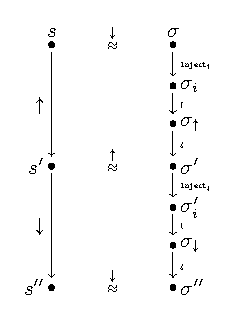
\includegraphics[keepaspectratio,width=.4\linewidth]{Figures/Proof/beh-preser-details}
  \caption{Bisimulation diagram over one clock cycle for a source
    SITPN and a target \hvhdl{} design.}
  \label{fig:bisim-diagram}
\end{figure}

Here, we present Lemma~\nameref{lem:re} and Lemma~\nameref{lem:fe},
along with their proofs. In the two lemmas, we added an extra
hypothesis about the starting state of the \hvhdl{} design:
$\mathcal{D}_{\mathcal{H}},\Delta,\sigma\vdash\mathrm{d.cs}\xrightarrow{comb}\sigma$. The
hypothesis states that all signal values are stable at the beginning
of the considered clock phase. This means that the execution of the
combinational part of the \hvhdl{} design does not change the value of
signals anymore. This hypothesis is mandatory to determine the
expression associated to combinational signals, i.e the combinational
equations, at the beginning of the clock phase (see
Section~\ref{sec:detailled-proof} for more details about combinational
equations).

To prove Lemmas~\nameref{lem:re} and \nameref{lem:fe}, one must show
that every point of the state similarity relation in the conclusion
holds.  For each point, the proof is given as a separate lemma that
the reader will find in Appendix~\ref{app:sem-preserv-proof}. The
proof strategy to show the equalities or equivalences laid out in the
state similarity relation follows the same two-fold pattern:

\begin{itemize}
\item First, reason on the SITPN structure and on the transformation
  function to determine the content of the target \hvhdl{} design.
\item Then, reason on the SITPN state transition relation and the
  \hvhdl{} ``simulation'' relations (i.e, the $\mathtt{Inject}_{clk}$,
  $\uparrow$, $\downarrow$ and $\rightsquigarrow$ relations) to
  establish the equality between the values coming from the SITPN
  world (i.e, marking, time counters, reset orders, etc. and also
  predicates) and the values of the signals declared in the \hvhdl{}
  design and in its internal component instances.
\end{itemize}

The application of this proof strategy will be detailled in
Section~\ref{sec:detailled-proof}.

%%%%%%%%%%%%%%%%%%%%%%%%%%%%%%%%%%%%%%%
%%%%%%%%%% RISING EDGE LEMMA %%%%%%%%%%
%%%%%%%%%%%%%%%%%%%%%%%%%%%%%%%%%%%%%%%

\begin{lemma}[Rising edge]
  \label{lem:re}
  For all $sitpn\in{}SITPN$, $d\in{}design$, $\gamma\in{}WM(sitpn,d)$,
  $E_c\in\mathbb{N}\rightarrow\mathcal{C}\rightarrow\mathbb{B}$,
  $\Delta\in{}ElDesign(d,\mathcal{D}_\mathcal{H})$,
  $E_p\in(\mathbb{N}\times\{\uparrow,\downarrow\})\rightarrow{}Ins(\Delta)\rightarrow{}value$,
  $\tau\in\mathbb{N}$, $s,s'\in{}S(sitpn)$,
  $\sigma_e,\sigma,\sigma_i,\sigma_\uparrow,\sigma'\in\Sigma(\Delta)$,
  assume that:
  \begin{itemize}
  \item $\lfloor{}sitpn\rfloor_\mathcal{H}=(d,\gamma)$ and
    $\gamma\vdash{}E_p\stackrel{env}{=}E_c$ and
    $\mathcal{D}_\mathcal{H},\emptyset\vdash\mathrm{d}\srarrow{elab}{\fontsize{7}{7}\selectfont}\Delta,\sigma_e$
  \item $\gamma\vdash{}s\stackrel{\downarrow}{\approx}\sigma$
  \item
    $E_c,\tau\vdash{}s\srarrow{\uparrow}{\fontsize{7}{7}\selectfont}s'$
  \item $\mathtt{Inject}_\uparrow(\sigma, E_p, \tau, \sigma_i)$ and
    $\mathcal{D}_{\mathcal{H}},\Delta,\sigma_i\vdash\mathrm{d.cs}\xrightarrow{\uparrow}\sigma_\uparrow$
    and
    $\mathcal{D}_{\mathcal{H}},\Delta,\sigma_\uparrow\vdash\mathrm{d.cs}\xrightarrow{\rightsquigarrow}\sigma'$
  \item State $\sigma$ is a stable design state:
    $\mathcal{D}_{\mathcal{H}},\Delta,\sigma\vdash\mathrm{d.cs}\xrightarrow{comb}\sigma$
  \end{itemize}
  then
  $\gamma,E_c,\tau\vdash{}s'\stackrel{\uparrow}{\approx}{}\sigma'$.
\end{lemma}

\begin{niproof}
  By definition of the \nameref{def:full-post-re-state-sim} relation,
  there are 8 points to prove:
  \begin{frameb}
    \begin{enumerate}
    \item
      $\forall{}p\in{}P,id_p\in{}Comps(\Delta)~s'.t.~\gamma(p)=id_p,$
      $~s'.M(p)=\sigma'(id_p)("s\_marking")$.\label{it:marking-eq-re}
    \item
      $\forall{}t\in{}T_i,id_t\in{}Comps(\Delta)~s.t.~\gamma(t)=id_t$,\\
      $\big(upper(I_s(t))=\infty\land{}s'.I(t)\le{}lower(I_s(t))\Rightarrow$
      $s'.I(t)=\sigma'(id_t)("s\_time\_counter")\big)$\\
      $\land\big(upper(I_s(t))=\infty\land{}s'.I(t)>{}lower(I_s(t))\Rightarrow$
      $\sigma'(id_t)("s\_time\_counter")=lower(I_s(t))\big)$\\
      $\land\big(upper(I_s(t))\neq\infty\land{}s'.I(t)>{}upper(I_s(t))\Rightarrow$
      $\sigma'(id_t)("s\_time\_counter")=upper(I_s(t))\big)$\\
      $\land\big(upper(I_s(t))\neq\infty\land{}s'.I(t)\le{}upper(I_s(t))\Rightarrow$
      $s'.I(t)=\sigma'(id_t)("s\_time\_counter")\big)$.\label{it:time-count-eq-re}
    \item
      $\forall{}t\in{}T_i,id_t\in{}Comps(\Delta)~s.t.~\gamma(t)=id_t,$
      $s'.reset_t(t)=\sigma'(id_t)("s\_reinit\_time\_counter")$.\label{it:reset-eq-re}
    \item
      $\forall{}a\in\mathcal{A},id_a\in{}Outs(\Delta)~s.t.~\gamma(a)=id_a,~s'.ex(a)=\sigma'(id_a)$.\label{it:action-eq-re}
    \item
      $\forall{}f\in\mathcal{F},id_f\in{}Outs(\Delta)~s.t.~\gamma(f)=id_f,~s'.ex(f)=\sigma'(id_f)$.\label{it:fun-eq-re}
    \item
      $\forall{}t\in{}T,id_t\in{}Comps(\Delta)~s.t.~\gamma(t)=id_t,$
      $t\in{}Sens(s'.M)\Leftrightarrow\sigma'(id_t)("s\_enabled")=\mathtt{true}$.\label{it:sens-eq-re}
    \item
      $\forall{}t\in{}T,id_t\in{}Comps(\Delta)~s.t.~\gamma(t)=id_t,$
      $t\notin{}Sens(s'.M)\Leftrightarrow\sigma'(id_t)("s\_enabled")=\mathtt{false}$.\label{it:not-sens-eq-re}
    \item
      $\forall{}t\in{}T,id_t\in{}Comps(\Delta)~s.t.~\gamma(t)=id_t,$\\
      $\sigma'(id_t)("s\_condition\_combination")=
      \prod\limits_{c\in{}conds(t)}
      \begin{cases}
        E_c(\tau,c) & if~\mathbb{C}(t,c)=1 \\
        \mathtt{not}(E_c(\tau,c)) & if~\mathbb{C}(t,c)=-1 \\
      \end{cases}$\\
      where
      $conds(t)=\{c\in\mathcal{C}~\vert~\mathbb{C}(t,c)=1\lor\mathbb{C}(t,c)=-1\}$.\label{it:cond-comb-eq-re}
    \end{enumerate}
  \end{frameb}
  
  Each point is proved by a separate lemma:
  \begin{itemize}[label=--]
  \item Apply Lemma~\nameref{lem:re-equal-marking} to solve
    \ref{it:marking-eq-re}.
  \item Apply Lemma~\nameref{lem:re-equal-tc} lemma to solve
    \ref{it:time-count-eq-re}.
  \item Apply Lemma~\nameref{lem:re-equal-reset-orders} to solve
    \ref{it:reset-eq-re}.
  \item Apply Lemma~\nameref{lem:re-equal-action-exec} to solve \ref{it:action-eq-re}.
  \item Apply Lemma~\nameref{lem:re-equal-fun-exec} to solve
    \ref{it:fun-eq-re}.
  \item Apply Lemma~\nameref{lem:re-equal-sens} to solve
    \ref{it:sens-eq-re}.
  \item Apply Lemma~\nameref{lem:re-equal-not-sens} to solve
    \ref{it:not-sens-eq-re}.
  \item Apply Lemma~\nameref{lem:re-equal-cond-comb} to solve
    \ref{it:cond-comb-eq-re}.
  \end{itemize}
\end{niproof}

\begin{lemma}[Falling edge]
  \label{lem:fe}
  For all $sitpn\in{}SITPN$, $d\in{}design$, $\gamma\in{}WM(sitpn,d)$,
  $E_c\in\mathbb{N}\rightarrow\mathcal{C}\rightarrow\mathbb{B}$,
  $\Delta\in{}ElDesign(d,\mathcal{D}_\mathcal{H})$,
  $E_p\in(\mathbb{N}\times\{\uparrow,\downarrow\})\rightarrow{}Ins(\Delta)\rightarrow{}value$,
  $\tau\in\mathbb{N}$, $s,s'\in{}S(sitpn)$,
  $\sigma_e,\sigma,\sigma_i,\sigma_\downarrow,\sigma'\in\Sigma(\Delta)$,
  assume that:
  \begin{itemize}
  \item $\lfloor{}sitpn\rfloor_\mathcal{H}=(d,\gamma)$ and
    $\gamma\vdash{}E_p\stackrel{env}{=}E_c$ and
    $\mathcal{D}_\mathcal{H},\emptyset\vdash\mathrm{d}\srarrow{elab}{\fontsize{5}{7}\selectfont}\Delta,\sigma_e$
  \item $\gamma,E_c,\tau\vdash{}s\stackrel{\uparrow}{\approx}\sigma$
  \item $E_c,\tau\vdash{}s\xrightarrow{\downarrow}s'$
  \item $\mathtt{Inject}_\downarrow(\sigma, E_p, \tau, \sigma_i)$
    and
    $\Delta,\sigma_i\vdash\mathrm{d.cs}\xrightarrow{\downarrow}\sigma_{\downarrow}$
    and
    $\Delta,\sigma_{\downarrow}\vdash\mathrm{d.cs}\xrightarrow{\rightsquigarrow}\sigma'$
  \item State $\sigma$ is a stable design state:
    $\mathcal{D}_{\mathcal{H}},\Delta,\sigma\vdash\mathrm{d.cs}\xrightarrow{comb}\sigma$
  \end{itemize}
  then $\gamma\vdash{}s'\stackrel{\downarrow}{\approx}{}\sigma'$.
\end{lemma}

\begin{niproof}
  By definition of the \nameref{def:post-fe-state-sim} relation, there
  are 11 points to prove:
  \begin{frameb}
    \begin{enumerate}
    \item
      $\forall{}p\in{}P,id_p\in{}Comps(\Delta)~s.t.~\gamma(p)=id_p,$
      $~s'.M(p)=\sigma'(id_p)("s\_marking")$.\label{item:fe-equal-marking}
    \item
      $\forall{}t\in{}T_i,id_t\in{}Comps(\Delta)~s.t.~\gamma(t)=id_t,$\\
      $\big(upper(I_s(t))=\infty\land{}s'.I(t)\le{}lower(I_s(t))\Rightarrow{}s'.I(t)=\sigma'(id_t)("s\_time\_counter")\big)$\\
      $\land\big(upper(I_s(t))=\infty\land{}s'.I(t)>{}lower(I_s(t))\Rightarrow{}\sigma'(id_t)("s\_time\_counter")=lower(I_s(t))\big)$\\
      $\land\big(upper(I_s(t))\neq\infty\land{}s'.I(t)>{}upper(I_s(t))\Rightarrow{}\sigma'(id_t)("s\_time\_counter")=upper(I_s(t))\big)$\\
      $\land\big(upper(I_s(t))\neq\infty\land{}s'.I(t)\le{}upper(I_s(t))\Rightarrow{}s'.I(t)=\sigma'(id_t)("s\_time\_counter")\big)$.
      \label{item:fe-equal-tc}
    \item
      $\forall{}c\in\mathcal{C},id_c\in{}Ins(\Delta)~s.t.~\gamma(c)=id_c,~s'.cond(c)=\sigma'(id_c)$.\label{item:fe-equal-cond-values}
    \item
      $\forall{}a\in\mathcal{A},id_a\in{}Outs(\Delta)~s.t.~\gamma(a)=id_a,~s'.ex(a)=\sigma'(id_a)$.\label{item:fe-equal-act-exec}
    \item
      $\forall{}f\in\mathcal{F},id_f\in{}Outs(\Delta)~s.t.~\gamma(f)=id_f,~s'.ex(f)=\sigma'(id_f)$.\label{item:fe-equal-fun-exec}
    \item
      $\forall{}t\in{}T,id_t\in{}Comps(\Delta)~s.t.~\gamma(t)=id_t,$
      $t\in{}Firable(s')\Leftrightarrow\sigma'(id_t)("s\_firable")=\mathtt{true}$.\label{item:fe-equal-firable}
    \item
      $\forall{}t\in{}T,id_t\in{}Comps(\Delta)~s.t.~\gamma(t)=id_t,$
      $t\notin{}Firable(s')\Leftrightarrow\sigma'(id_t)("s\_firable")=\mathtt{false}$.\label{item:fe-equal-not-firable}
    \item
      $\forall{}t\in{}T,id_t\in{}Comps(\Delta)~s.t.~\gamma(t)=id_t,$
      $t\in{}Fired(s')\Leftrightarrow\sigma'(id_t)("fired")=\mathtt{true}$.\label{item:fe-equal-fired}
    \item
      $\forall{}t\in{}T,id_t\in{}Comps(\Delta)~s.t.~\gamma(t)=id_t,$
      $t\notin{}Fired(s')\Leftrightarrow\sigma'(id_t)("fired")=\mathtt{false}$.\label{item:fe-equal-not-fired}
    \item
      $\forall{}p\in{}P,id_p\in{}Comps(\Delta)~s.t.~\gamma(p)=id_p,$
      $\sum\limits_{t\in{}Fired(s')}pre(p,t)=\sigma'(id_p)("s\_output\_token\_sum")$.\label{item:fe-equal-ots}
    \item
      $\forall{}p\in{}P,id_p\in{}Comps(\Delta)~s.t.~\gamma(p)=id_p,$
      $\sum\limits_{t\in{}Fired(s')}post(t,p)=\sigma'(id_p)("s\_input\_token\_sum")$.\label{item:fe-equal-its}
    \end{enumerate}
  \end{frameb}

  Each point is proved by a separate lemma:
  \begin{itemize}[label=--]
  \item Apply Lemma~\nameref{lem:fe-equal-marking} to solve
    \ref{item:fe-equal-marking}.
  \item Apply Lemma~\nameref{lem:fe-equal-tc} to solve
    \ref{item:fe-equal-tc}.
  \item Apply Lemma~\nameref{lem:fe-equal-cond-values} to solve
    \ref{item:fe-equal-cond-values}.
  \item Apply Lemma~\nameref{lem:fe-equal-act-exec} to solve
    \ref{item:fe-equal-act-exec}.
  \item Apply Lemma~\nameref{lem:fe-equal-fun-exec} to solve
    \ref{item:fe-equal-fun-exec}.
  \item Apply Lemma~\nameref{lem:fe-equal-firable} to solve
    \ref{item:fe-equal-firable}.
  \item Apply Lemma~\nameref{lem:fe-equal-not-firable} to solve
    \ref{item:fe-equal-not-firable}.
  \item Apply Lemma~\nameref{lem:fe-equal-fired} to solve
    \ref{item:fe-equal-fired}.
  \item Apply Lemma~\nameref{lem:fe-equal-not-fired} to solve
    \ref{item:fe-equal-not-fired}.
  \item Apply Lemma~\nameref{lem:fe-equal-ots} to solve
    \ref{item:fe-equal-ots}.
  \item Apply Lemma~\nameref{lem:fe-equal-its} to solve
    \ref{item:fe-equal-its}.
  \end{itemize}
\end{niproof}


%%% Local Variables:
%%% mode: latex
%%% TeX-master: "../../main"
%%% End:
